\documentclass[oneside,12pt,fleqn]{memoir}
\usepackage{makeidx}
%\usepackage[utf8]{inputenc}
\pagestyle{plain}
%%%%%%%%%%%%%%%%%%%%%%%%%%%%%%%%%%% importa pacchetti
\usepackage{usepkg}
\usepackage{fancyfoot}
%%%%%%%%%%%%%%%%%%%%%%%%%%%%%%%%%%%%%
%%%%%%%%%%%%%%%%%% titletoc, titlesec setting
\usepackage{titleT}
%%%%%%%%%%%%%%%%%% setlength
\usepackage{mylength}
\linespread{0.5}
%%%%%%%%%%%% Hyperref package
\usepackage{hyperref}
\hypersetup{
    colorlinks,
    citecolor=black,
    filecolor=black,
    linkcolor=black,
    urlcolor=black
}
%%%%%%%%%%%%%%%%%%%%%%%%
%%%%%%%%%%%%%%%%%Geometry package
\usepackage{mygeometry}
%%%%%%%%%%%%%%%%%%%%%%%%%%%%%%%%%%% Funzioni per questo file main
\usepackage{LocalF}
%%%%%%%%%%%%%%%%%%%%%%%%%%%%%%%%%%% Funzioni generali
\usepackage{functions}
\usepackage{mathOp}
%http://tex.stackexchange.com/questions/246/when-should-i-use-input-vs-include
\usepackage{sources}
%%%%%%%%%%%%%%%%%%%%%%%%%%%%%%%%%

\makeindex
\raggedbottom %http://tex.stackexchange.com/questions/102084/annoying-paragraph-spacing-issue-with-memoir

\author{Pippetta}
\titleSounti per tesi eliosismologia}
\date{\today}

\begin{document}

\frontmatter


\maketitle


\tableofcontents*
\listoffigures

\mainmatter



\part{Cosa fare?

\subfile{intro}

\part{Tesina}

\subfile{helioSSMintro}

\subfile{waves}

\chapter{Problema inverso: correzione al modello dalle oscillazioni.}
\PartialToc

\section{Per punti.}

\begin{itemize}
    
    \item astratto forme di inversione: 3 tipi. Primary inversion: asymptotic technique. Secondary inversion: impose thermal equilibrium, energy transport, equation of state, $\kappa$, $\epsilon$. Tertiary inversion impose that the evolution of the Sun is in accordance with standard model. Inversione fornisce dettagli sulla ''microfisica''.
    
    \item By determining frequency of p,g modes we can probe variation of $c(r)$ and $N$.
    \item Principio variazionale
    \item Tesseral modes ($m\neq0$) yield information about Sun's internal rotation and magnetic field (justified ignoring effects of centrifugal and Lorentz force on radial structure)
    \item Variational principle, model dependent inverion methods. Non ''perfetta corrispondenza'' nel modello solare.
    
    \item Rotation: relation data vs $\Omega(r)$ is linear to high approximation
    \begin{equation*}
    \Delta_i=\int_0^RK_i(r)\Omega(r)\,dr+\epsilon_i
    \end{equation*}
    $\Delta_i$ sono le frequenze osservate e $\epsilon_i$ l'errore sulle frequenze osservate.
    
    \item Dzi90: pressure, density in neutrino production regions: knowledge of these thermodynamic function doesn't suffice tpo determine T.
    
    \item Inversion methods: JCD85; Brodsky, Vorontsov 88; JCD, Gough, Thompson 88;  Vorontsov 88; Kosovichev 88; Gough Kosovichev 88.
    
    \item In determinati casi \'e sufficiente confrontare le differenze di frequenza $\delta_{nl}=\nu_{n,l}-\nu_{n-1,l+2}$ piuttosto che le frequenze assolute.
    
    \item Asymptotic method is not valid in innermost part of the Sun: Shibahashi sekii 88 (shart wavelength asymptotic); shibahashi 89; JCD 89 
    
    \item In the structure case relation between structure and multiplet is highly nonlinear.
    \item Exactly calculated eigenfunction: linearization about SSM.
    \item Averaged  multiplet $\nu_{nl}$ carry info about sherical symmetric component of solar structure: testin solar model, info about properties of matter in solar interior.
    \item $\Gamma_1$, $\rho$, $c$ are constrained by freq. directly.
    \item If equation of state and heavy elements abundances are known $\Gamma_1$ can be expressed in terms of a thermodynamical variable and $Y$: $(\frac{P}{\rho},Y)$, $(\rho,Y)$.
    
    \item Gough84:  Inversion of $F(w)$: $c(t)$ without reference to the model.
    
    \item Simple form of asymptotic analysis
    \begin{align*}
    &\frac{\pi(n+\alpha)}{\omega}\approx F(\frac{\omega}{L})\\
    &F(w)=\int_{r_t}^R\sqrt{1-\frac{c^2}{w^2r^2}}\frac{dr}{c}
    \end{align*}
    sistematic error.
    \item differential asymptotic inversion:
    \begin{align*}
    &S_{nl}\frac{\delta\omega_{nl}}{\omega_{nl}}\approx H_1(\frac{\omega_{nl}}{L})+H_2(\omega_{nl})\\
    &S_{nl}=\int_{r_t}^R(1-\frac{L^2c^2}{r^2\omega_{nl}^2})\expy{-\frac{1}{2}}\frac{dr}{c}-\pi\TDy{\omega}{\alpha}\\
    &H_1(w)=\int_{r_t}^R(1-\frac{c^2}{r^2w^2})\expy{-\frac{1}{2}}\frac{\delta_rc}{c}\frac{dr}{c}\\
    &H_2(w)=\frac{\pi}{\omega}\delta\alpha(\omega)
    \end{align*}
    
    \begin{figure}[!ht]
    \centering
    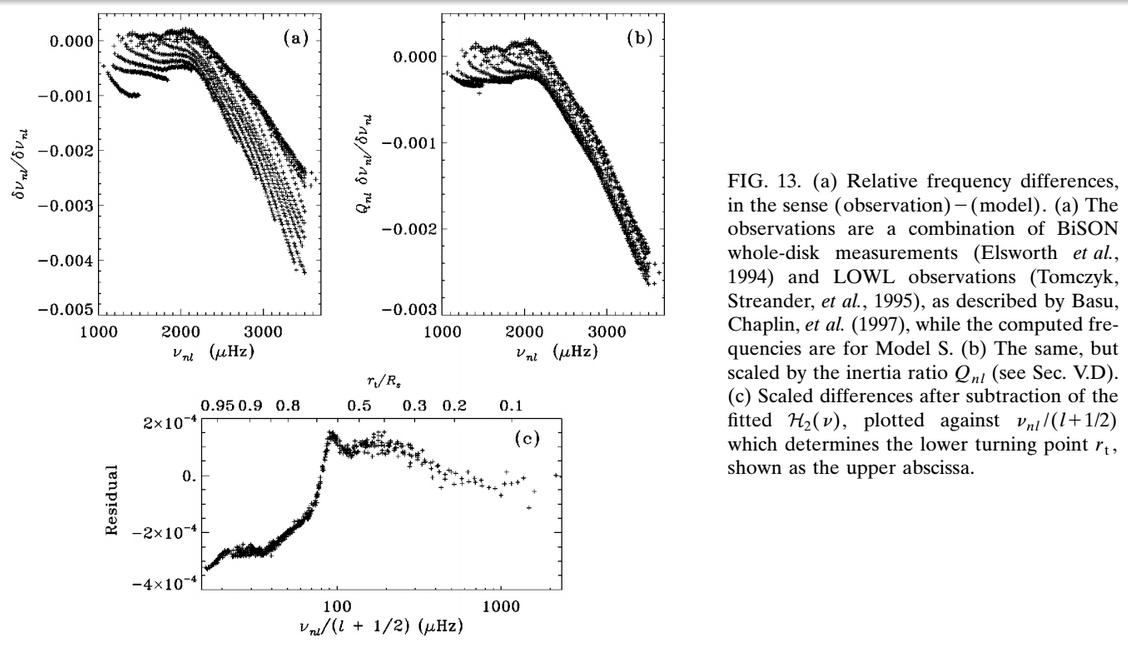
\includegraphics[width=\textwidth, height=0.9\textheight,keepaspectratio]{freqdiff_13}
    \caption{Frequency difference.}
    \end{figure}

    \clearpage
    
    Drastic change of behaviour for mode penetrating beneath base of convection zone
    
    \item $\nu$ sensitive to details of EOS (Berthomieu, lubow 80)
    \item Confronto densit\'a, velocit\'a del suono del modello vs quelle ottenute dalle frequenza misurate
    \item Frequency changes as linear functional of properties of the models (vedi stix 5.3 etc) for small changes.
    \item Changes to the properties of the model are directly infered from observations.
    \item tecniche di inversion. Classe coefficienti lineare: mola, sola, inversion of acustic data (Thomson 1993). Classe parametri lineare: regularized least square,statistical properties of inference from inversion.
    \item Result of inversion using SOLA fig 14
    \item Inversion technique to deduce interior structure and dynamics given frequencies and their splitting.
    \item Inside of our nearest star as gleaned from the study of its vibration.
    \item Fornisce strumente per scoprire dove il modello solare \'e deficitario (correzioni alla legge dei gas perfetti, Z, etc)
    \item chemical constitution low l p modes (Jimenez88, noel84).
    \item EOS: Electrostatic correct5ion to PG law (Debye-Huckel theory). Effects of electrostatic corrections upon eigenvalue spectrum of low degree p modes + Partial electron degeneracy.
    \item Gli aspetti della struttura solare sono determinati direttamente dai dati.
    \item Determinazione struttura idrostatica.
    \item Inversion of dynamical oscillation: relation between pressure and inertia density $\rho$.
    \item $\omega_{n,l}-\omega_{n-1,l+2}$: chemical inhomogeneities.
    \item Error to be assigned to helioseismological determination of physical quantities Q (characterizing solar structure).
    \item Errors evaluation: Var/CoVar matrix.
\end{itemize}


\section{Tecniche asintotiche.}

Per modi di basso grodo \'e possibile espandere al primo ordine l'integrale nella \ref{eq:duvall} $F(w)\approx\int_0^R\frac{dr}{c}-w\expy{-1}\frac{\pi}{2}$ ed esprimere la legge di Duvall tramite
\begin{equation}\label{eq:claverie}
    \nu_{nl}=\frac{\omega_{nl}}{2\pi}\approx(n+\frac{l}{2}+\frac{1}{4}+\alpha)\Delta\nu
\end{equation}
con $\Delta\nu=[\int_0^R\frac{dr}{c}]\expy{-1}$.
La presenza di picchi uniformemente spaziati di modi a basso grado l \'e stata osservata da Cleverie79.

Estendendo ancora l'espansione di \ref{eq:duvall} si ha una misura della variazione di $c$ nel core della stella
\begin{equation}\label{eq:tassoul}
    d_{nl}=\nu_{nl}-\nu_{n-1,l+2}\approx-(4l+6)\frac{\Delta\nu}{4\pi^2\nu_{nl}}\int_0^R\frac{dc}{dr}\frac{dr}{r}
\end{equation}
La velocit\'a del suono \'e ridotta a causa dell'aumentare di $\mu$ durante la fusione di H in He durante l'evoluzione stellare e quindi $d_{nl}$ \'e ridotto.

\begin{todo}{Analisi legge Duval }
Dalsnotes Pg 155
\end{todo}

\section{Linearizzazione della ''variazione'' attorno ad un modello solare.}

\subsection{Principio variazionale}

Riscrivo l'equazione del moto linearizzata nella forma
\begin{equation}
    \omega^2\Lvar{\vec{r}}=\frac{1}{\rho}\nabla p'-\vec{g}'-\frac{\rho'}{\rho}\vec{g}=\mathcal{F}(\Lvar{\vec{r}})
\end{equation}
da cui risulta che in seguito ad una perturbazione del modello di equilibrio $\Lvar{\mathcal{F}}$ le frequenze delle oscillazioni adiabatiche sono determinate da 

\begin{equation}\label{eq:variational}
    \Lvar{\omega^2}=\frac{\int_V\Lvar{\vec{r}}^*\cdot\mathcal{F}(\Lvar{\vec{r}})\rho\,dV}{\int_V|\Lvar{\vec{r}}|^2\rho\,dV}
\end{equation}
$\Lvar{\vec{r}}$ \'e autovalore per il problema imperturbato.




\section{Rotazione.}

Il Sole \'e un rotatore lento.



We want to find a velocity field which in spherical coordinates has the form
\begin{align*}
&\vec{v_0}=(0,0,r\Omega\sin{\theta})=\vecp{\Omega}{r}\\
&\vec{\Omega(r,\theta)}=(\Omega(r,\theta)\cos{\theta},-\Omega(r,\theta)\sin{\theta},0)&\intertext{il vettore velocit\'a angolare \'e funzione di r e $\theta$}
\end{align*}

Without rotation the inertia term is $\rho_0\TDy{t}{\vec{v}}=\rho_0\PtwoDy{t}{\vec{\xi}}$ where there is no mean motion, in case of rotation $\rho_0(\PDof{t}+\scap{v_0}{\nabla})^2\vec{\xi}$.

We consider additional term as a small perturbation

\begin{align*}
&\PDof{t}=i\omega\\
&\omega=\omega_{\alpha}+\Delta\omega_{\alpha}\\
&Y_{\alpha}=Y_{lm}\\
&\rho_0(\omega_{\alpha}^2+2\omega_{\alpha}\Delta\omega_{\alpha})\vec{\xi}\\
&=\nabla P_1-\frac{\rho_1}{\rho_0}\nabla P_0+\rho_0\nabla\Phi_1+2i\omega_{\alpha}\rho_0(\scap{v_0}{\nabla})\vec{\xi}&\intu{equazione del moto al primo ordine nella perturbazione}
\end{align*}

quindi risulta

\begin{align*}
&\Delta\omega_{\alpha}=\frac{i\int\rho_0\xi_{\alpha}^*(\scap{v_0}{\nabla})\xi_{\alpha}}{\int\rho_0\xi_{\alpha}^*\xi_{\alpha}}\\
&\Delta\omega_{\alpha}=\frac{-m\int\rho_0\Omega\xi_{\alpha}^*\xi_{\alpha}\,dV+i\int\rho_0\xi_{\alpha}^*(\vecp{\Omega}{\xi_{\alpha}})\,dV}{\int\rho_0\xi_{\alpha}^*\xi_{\alpha}}\intu{usando $\vec{v_0}=\vecp{\Omega}{r}$}
\end{align*}

Dobbiamo trovare $\Omega(r,\theta)$ dalla differenza $\Delta\omega_{\alpha}$: the problem is linear in $\Omega$ so the shift $\Delta\Omega_{\alpha}$ is of the same order as $\Omega$.

For evaluation of shift formula we must know eigenfunction $\xi_{\alpha}$ of unperturbed state.

Per rotazione puramente radiale $\Omega(r)$
\begin{align*}
&\Delta\omega_{\alpha}=-m\frac{\int_0^{\rsun{}}\rho_0\Omega\{|\xi_r-\xi_h|^2+[l(l+1)-2]|\xi_h|^2\}r^2\,dr}{\int_0^{\rsun{}}\rho_0\{|\xi_r|^2+l(l+1)|\xi_h|^2\}r^2\,dr}\\
&=\int_0^{\rsun{}}K_{\alpha}(r)\Omega(r)\,dr
\end{align*}

nel caso di rotazione dipendente solo da r $\Delta\omega_{\alpha}$ \'e lineare in m, $2l+1$ frequencies with equidistant spacing.

Any given $\Delta\Omega_{\alpha}$ samples angular velocity in the depth range corresponding to $\xi_{\alpha}$.

Le osservazioni della superficie mostrano una dipendenza dalla co-latitudine 

\begin{equation*}
\frac{\Omega(\theta)}{2\pi}=\SI{451.5}{\nano\hertz}-\SI{65.3}{\nano\hertz}\cos^2{\theta}-\SI{66.7}{\nano\hertz}\cos^4{\theta}
\end{equation*}

risultato di un best fit (discrepanze notevoli e variazioni temporali).

For an investigation of the full function $\Omega(r,\theta)$ the whole multiplet $2l+1$ frequencies must be used: deviation from equidistant spacing within the multiplet is typical of latitudinal shear.


\section{Inversione non asintotica.}

In the structure case the relation between structure and multiplet frequencies is highly nonlinear: we perform linearization on the assumption that a solar model close enough to actual solar structure exists.

\subsection{Correzioni struttra idrostatica}

\'E possibile quindi mettere in relazione la differenze tra le frequenze osservate  con quelle calcolate da un modello, $\delta\omega_{nl}=\Omega_{\odot}-\Omega_{Mod}$ e le differenze nella stratificazione idrostatica

\begin{align}
&\frac{\delta\omega_{nl}}{\omega_{nl}}=\int_0^R[K^{nl}_{c^2,\rho}(r)\frac{\delta_rc^2}{c^2}(r)+K^{nl}_{\rho,c^2}(r)\frac{\delta_r\rho}{\rho}(r)]\,dr\\
&+I_{nl}\expy{-1}F_{Surf}(\omega_{nl})\\
&\frac{\delta_rc^2}{c^2}(r)=\frac{[c_{\odot}^2(r)-c_{mod}^2(r)]}{c^2(r)}\\
&\frac{\delta_r\rho}{\rho}(r)=\frac{[\rho_{\odot}(r)-\rho_{mod}(r)]}{\rho(r)}\label{eq:invstructure}
\end{align}

i kernel $K_Q^j$ dipendono dalle autofunzioni del modello, il termine $I_{nl}\expy{-1}F_{Surf}(\omega_{nl})$, $I_{nl}=\int_V|\Lvar{\vec{r}}|^2\rho\,dV$ \'e una correzione dovuta alle differenti condizioni fisiche che si incontrano vicino alla superficie: per basse frequenze si ha riflessione pi\'u in profondit\'a a $\omega=\omega_c$ e quindi risentono meno degli effetti degli strati superficiali.

The analysis in terms of $\frac{\delta_rc^2}{c^2}(r)$ and $\frac{\delta_r\rho}{\rho}(r)$ capture the difference between Sun and model related hydrostatic structure.

\subsection{Correzioni equazione di stato e composizione.}

Since sound speed depends upon $\Gamma_1$ as $c_s^2=\Gamma_1\frac{P}{\rho}$ we can express $\Gamma_1(P,\rho,Y,Z)$ from thermodynamic properties and composition of the gas.

We obtain equivalent formulation of \ref{eq:invstructure} expressing $\delta_rc^2$ in terms of $\delta_rP$, $\delta_r\rho$, $\delta_rY$ and $\delta_r\Gamma_1$

\begin{align}
&\frac{\delta\omega_{nl}}{\omega_{nl}}=\int_0^RK^{nl}_{u,Y}(r)\frac{\delta_ru}{u}(r)\,dr+\int K^{nl}_{Y,u}(r)\delta_rY\,dr\\
&+\int_0^RK^{nl}_{c^2,\rho}(r)(\frac{\delta\Gamma_1}{\Gamma_1})_{int}\,dr+I_{nl}\expy{-1}F_{Surf}(\omega_{nl})\label{eq:diffthermo}&\intertext{allowance in error $(\delta\Gamma_1)_{int}$, difference between $\Gamma_1$ Sun and $\Gamma_1$ model EOS.}
\end{align}

Fatti:
\begin{itemize}
    \item Inversione di $\Gamma_1$ mostra la necessit\'a di tener conto degli effetti relativistici per gli elettroni (average thermal energy approx \SI{1.35}{\kilo\ev} approx $0.3\%$ of $m_e$).
\end{itemize}


\section{(Numerical) Inversion technique.}

\subsection{Least square inversion.}

Parametrize unknown functions $\frac{\delta_rc^2}{c^2}$, $\frac{\delta_r\rho}{\rho}$, $F_{Surf}$ (Slowly variable polynomials), the parameter being determined through regularized least square fitting (Dziembowski90, Antia Basu 94).

\subsubsection{(Regularized least square methods)}
(JCD90).

\subsection{(OLA)}
(Backus, Gibbert 68,70; Gough 85).

%For rotation inversion $\omega=\omega_{0nl}+m\omega_{1nl}$, $\omega_{1nl}=\int_0^1K_{nl}(x)\Omega(x)\,dx+\epsilon_{nl}$ con $x=\frac{r}{R}$ e $\epsilon_{nl}$ errori in $\omega_{1nl}$
%$\ensemble{c_i(r_0)}$

\subsection{SOLA}
(Pijpers, thompson 92).

Let's determine $\frac{\delta_rc^2}{c^2}$

Expression to be minimized

\begin{align*}
&\int_0^R[\mathcal{K}_{c^2,\rho}(r_0,r)-\mathcal{T}(r_0,r)]^2\,dr\\
&+\beta\int_0^R\mathcal{G}_{\rho,c^2}(r_0,r)\,dr+\mu\sum_i\sigma_ic_i(r_0)c_j(r_0)\\
&\mathcal{K}_{c^2,\rho}(r_0,r)=\sum_ic_i(r_0)K_{c^2,\rho}^i(r)&\intu{averaging kernel}\\
&\mathcal{G}_{\rho,c^2}(r_0,r)=\sum_ic_i(r_0)K_{\rho,c^2}^i(r)&\intu{cross-term kernel which controls the undesidered contrib from $\frac{\delta_r\rho}{\rho}$}
\end{align*}

dove $i=(n,l)$ e $\sigma_i$ \'e l'errore su $\frac{\delta\omega_i}{\omega_i}$.

In general we choose coefficient $c_i(r_0)$ such that $\sum c_i(r_0)\frac{\delta\omega_i}{\omega_i}$ provides a localized average of $\frac{\delta f_1(r)}{f_1(r)}$ around $r=r_0$:

\begin{align*}
&\sum_ic_i(r_0)\frac{\delta\omega_i}{\omega_i}=\int_0^R\sum_ic_i(r_0)K_{1,2}^i(r)\frac{\delta f_1(r)}{f_1(r)}\,dr\\
&+\int_0^R\sum_ic_i(r_0)K_{2,1}^i(r)\frac{\delta f_2(r)}{f_2(r)}\,dr\\
&+\sum_ic_i(r_0)\frac{F_{Surf}(\omega_i)}{\omega_i}
\end{align*}

First term is an average of $\frac{\delta f_1}{f_1}$ weighted by a kernel $\mathcal{K}(r,r_0)=\sum_ic_i(r_0)K_{1,2}^i(r)$.

Second terms is the influence of second function on the solution of the first: weighting function $\mathcal{L}_{21}(r_0,r)=\sum_ic_i(r_0)K_{21}^i(r)$.

The third term is the influence of surface.

The coefficient $c_i(r_0)$ are selected to resmble target function, minimize contamination from $\frac{\delta f_2}{f_2}$ via $\mathcal{L}_{21}$ and minimize effect of noise:

are choosen to minimize
\begin{align*}
&\int(\sum_ic_iK_{12}^i)^2\,dr
&+\beta\int(\sum_ic_iK_{21}^1)^2\,dr\\
&+\mu\sum_{ij}c_ic_jE_{ij}
\end{align*}

$\beta$ is a parameter for contribution of second term.

\section{Helioseismic constrain on solar structure}
We use a SSM as starting model about which hydrostatic equations are linearized: see variational principle connecting differences between solar and the model function describing radial structure to corresponding differences in modes frequencies.

From inversion we infer the value of observables 

\begin{align*}
&Q_{\odot}=Q_{Mod}+q(\omega)&\intertext{for a given inversion procedure $\Delta\Omega$ propagate to the helioseismic value of observable $Q_{\odot}$, also we a residual dependence on starting model and regularization procedure}
\end{align*}


Asymptotic approximation for radial eigenfunction (integral equation connectin sound speed $c(r)$ to $\Omega_{nl}$) is inadequate (especially in deep interior)

\subsection{Helioseismological ''correction'' procedure}

\begin{itemize}
\item $\{\Omega\}$ of p-modes $\xrightarrow{\text{inversion}}Q$.
\item Solar Model $\to Q_{Mod}\to \{\Omega_{Mod}\}$.
\item $\Omega_{Mod}$ vs $\Omega_{\odot}\pm\Delta\Omega_{\odot}$: searching for correction q to solar model in order to match $\{\Omega_{Mod}+\omega(q)\}\leftrightarrow\Omega_{\odot}$. ($\omega(q)$: linear perturbation theory)
\end{itemize}

Assumptions:
\begin{align*}
&q=Q_{\odot}-Q_{Mod}\\
&\gamma=\Gamma_{\odot}-\Gamma_{Mod}&\intertext{$P, \rho$ and combination of their derivatives: connected through linearized mechanical equilibrium condition}
\end{align*}

\begin{itemize}
\item Slow variation of unknown functions
    \item Using a thermodynamical relation for $\Gamma(P,\rho,Y)$ one can eliminate one of the functions $q(x),\gamma(x), F(\Omega)$ and assuming $Y=Y_{ph}$ in convection zone and $\gamma=0$ in radiative interior
\end{itemize}


with these additional constraints the unknown function $\gamma$ is related with unknown number $Y_{ph}^{\odot}$, and chosing $U=\frac{P}{\rho}$ we write \autoref{eq:diffthermo}, where
\begin{itemize}
    \item $\delta_ru=u_{\odot}-U_{Mod}=u$.
    \item $y_{ph}=Y_{ph}^{\odot}-Y_{ph}^{mod}$.
\end{itemize}

\subsection{Outer convective zone.}

The quantities characterizing the outer part are $R_b$, $Y_{ph}$ and $c_b$, $\rho_b$ at bottom of convection zone.

\begin{itemize}
    \item He abundance. Helioseismical detemination $Y_{ph}=\numrange{0.226}{0.260}$.
    
    \item Bottom of convection zone.
    
    Transition of temperature gradient between subadiabatic and adiabatic at base of solar convection zone gives rise to clear signature in sound speed: helioseismical measurement of sound speed permits determination of base of convection zone
    
    \begin{align*}
    &\frac{R_b}{\rsun{}}=\numrange{0.710}{0.716}\\
    &c_b=\SIrange{0.221}{0.225}{\mega\meter\per\second}
    \end{align*}
    
    Lower part of convective zone is very close to being adiabatically stratified, $\Gamma\approx\frac{5}{3}$: $P\propto\rho\expy{\frac{5}{3}}$.
    
    $\rho_b$ is an indipendent quantity ($\rho(x)$ in convective zone is determined up to a scaling factor): the helioseismological determination of $\rho_b$ fixes such a factor.
    
    \begin{equation*}
        \rho_b=\SI{0.192}{\gram\per\cubic\cm}
    \end{equation*}
    
\end{itemize}

\subsection{Intermediate part ($0.2<x<0.65$)}

Isothermal sound speed $U=\frac{P}{\rho}$: recostruction of sound speed profile $c^2=\Gamma U$.

Below convective zone $\Gamma=\frac{5}{3}$ with an accuracy of \num{e-3} or better. Helioseis. determination is very accurate in this region $\frac{\Delta U}{U}\leq5 \perthousand$.

\subsection{Inner part ($x<0.2$)}

\appendix
\part{Appendice}

\stopcontents[chapters]


\clearpage
\addcontentsline{toc}{section}{Index}
\printindex

\end{document}